\documentclass[12pt,a4paper,openright,twoside]{book}
\usepackage[utf8]{inputenc}
\usepackage{disi-thesis}
\usepackage{code-lstlistings}
\usepackage{notes}
\usepackage{shortcuts}
\usepackage{acronym}

\school{\unibo}
\programme{Corso di Laurea Magistrale in Ingegneria e Scienze Informatiche}
\title{Fancy Title}
\author{Francesco Magnani}
\date{\today}
\subject{Software Process Engineering}
\supervisor{Danilo Pianini}
\cosupervisor{Nicolas Farabegoli}
\morecosupervisor{Angela Cortecchia}
\session{III}
\academicyear{2023-2024}

% Definition of acronyms
\acrodef{IoT}{Internet of Thing}
\acrodef{vm}[VM]{Virtual Machine}
\acrodef{IDE}[IDE]{Integrated Development Environment}
\acrodef{CI}[CI]{Continuous Integration}
\acrodef{AST}[AST]{Abstract Syntax Tree}
\acrodef{KAPT}{Kotlin Annotation Processing Tool}
\acrodef{KSP}{Kotlin Symbol Processing}
\acrodef{IR}{Intermediate Representation}


\mainlinespacing{1.241} % line spacing in mainmatter, comment to default (1)

\begin{document}

\frontmatter\frontispiece

\begin{abstract}	
Max 2000 characters, strict.
\end{abstract}

\begin{dedication} % this is optional
Optional. Max a few lines.
\end{dedication}

%----------------------------------------------------------------------------------------
\tableofcontents   
\listoffigures     % (optional) comment if empty
\lstlistoflistings % (optional) comment if empty
%----------------------------------------------------------------------------------------

\mainmatter

%----------------------------------------------------------------------------------------
\chapter{Introduction}
\label{chap:introduction}
%----------------------------------------------------------------------------------------

Analyzing characteristics of the source code without necessarily building and
executing it (i.e., static analysis) is a process that has been studied and
implemented in various forms during the last decades. Various tools have been
developed to perform such a task, each with its own strengths and weaknesses.
%
The need for such a tool is often evident in the software development process,
where ensuring the \textbf{quality} and \textbf{robustness} of software systems
is a critical concern. Using code quality analysis techniques is also a powerful
mean to avoid situations of ``technical debt''
\cite{DBLP:conf/sigsoft/ErnstBONG15}, that targets the system quality in
maintenance and evolution.

As the system grows in complexity, so does the variety of errors and
vulnerabilities that can be detected through tools (e.g., concurrency management
issues, error handling, etc.). At the same time, adhering to coding standards
helps to avoid both trivial and non-trivial errors from the outset.
Additionally, these are among the easiest types of tools to integrate, often
already included within \acp{IDE}.
%
The effectiveness of static analysis tools has been the subject of various
studies,  \cite{DBLP:journals/jss/LenarduzziPSLP23} evaluating their detection
capabilities, agreement, and precision. Some of these studies revealed a low
degree of agreement among the tools and highlighted the need for a better
understanding of their actual capabilities. More advance tools have been used
also to rewrite code and help with the development of very complex systems,
like \emph{Coccinelle} for the Linux kernel
\cite{DBLP:conf/eurosys/PadioleauLHM08}\cite{DBLP:conf/usenix/LawallM18}.
%
More over, in the last years, the static analysis tools have become more popular
and easier to use, becoming protagonists of many \ac{CI} pipelines
\cite{DBLP:conf/msr/ZampettiSOCP17} that automatically performs checks on the
entire source code, embracing change and evolution of the software without
making it a threat \cite{DBLP:books/daglib/0015650}, backed by a solid safety
net.

If looked from another perspective, automated static analysis tools and
compilers share significant similarities in their operations. Both perform
thorough examinations of source code without executing it, aiming to identify
errors, enforce coding standards, and optimize performance. Most of what
compilers do on the static analysis side is to facilitate code optimization and
error detection during the compilation process. In fact, a compiler can be
viewed as a form of static analysis tool, as it analyzes code to generate
executable programs and associated debugging information
\cite{DBLP:journals/queue/Thomson21}.
%
Specialized static analysis tools, on the other hand, extend beyond the
capabilities of standard compilers by offering additional functionalities and
broader diagnostic capabilities. They offer a broader range of diagnostic rules,
enabling the detection of specific and uncommon bugs that compilers might
overlook.
%
What if, however, the compiler were extended beyond its core functionality,
incorporating specialized capabilities that go beyond the scope of a
general-purpose environment? These extensions could be designed to address the
unique requirements of a specific project or domain. This is precisely where
\textbf{compiler plugins} come into play.

\section{Definition and Purpose of Compiler Plugins}

Compiler plugins are dynamic modules that interact with the compiler during its
various phases, enabling the introduction of new functionalities or the
modification of existing behaviors. They serve as intermediaries that can
inspect, modify, or enhance the compilation process, providing developers with
the flexibility to implement domain-specific checks, optimizations, or
transformations, all without altering the compiler's core architecture. 
%
For instance, in the context of the GNU Compiler Collection
(GCC), plugins allow for the addition of new features without necessitating
modifications to the compiler itself (mostly, again, for optimization purposes).

\subsection{Types of Compiler Plugins}

Compiler plugins can be broadly categorized based on the phase of compilation they target:

\begin{itemize}
  \item \textbf{Frontend Plugins}: These plugins operate during the initial
  stages of compilation, focusing on tasks such as syntax analysis, semantic
  analysis, and intermediate representation generation. They are useful also for
  implementing custom syntax extensions, enforcing coding standards, or
  performing static code analyzes. For example, in the \emph{Rust} programming
  language, compiler plugins can introduce new syntax extensions and lint
  checks. 

  \item \textbf{Backend Plugins}: Functioning in the latter stages of
  compilation, backend plugins are concerned with code optimization, machine
  code generation, and platform-specific adjustments. They can be utilized to
  implement custom optimizations, support additional hardware
  architectures and more.
\end{itemize}

\subsection{Compiler Plugins in Kotlin}

Kotlin, a statically typed programming language developed by JetBrains, offers
robust support for compiler plugins, allowing developers to highly customize the
compilation process to their specific needs. 
%
Kotlin's compiler architecture facilitates the creation of plugins that can
modify or extend its behavior during compilation. For example, the
\emph{all-open} compiler plugin in Kotlin allows classes annotated with a
specific annotation to be open without the explicit \lstinline{open} keyword,
adapting Kotlin to the requirements of frameworks that need classes to be
open. 

When guiding developers towards the creation of compiler plugins, JetBrains
compares them to \textbf{Annotation Processors}
\cite{JetBrains:KotlinCompilerPlugin}. Annotation processors are a powerful
feature in many modern programming languages, including Java and Kotlin, that
allow developers to generate code, validate code, and perform various
compile-time checks based on \textbf{annotations} present in the source code.
%
In Java, annotation processors are part of the Java Compiler API and can be used
to generate additional source files, validate the correctness of the code, and
even modify the \ac{AST} of the code being compiled. They are
commonly used in frameworks and libraries to reduce boilerplate code and enforce
coding standards.
%
Kotlin also supports annotation processors through the \ac{KAPT} — which is, in
fact, a compiler plugin itself — that allows Kotlin code to interoperate with
Java annotation processors and, more recently, the \ac{KSP}, another compiler
plugin introduced as ``an API that you can use to develop lightweight compiler
plugins''. The former enables developers to leverage existing Java annotation
processors in their Kotlin projects and the latter, on the other hand, provides
a more efficient and Kotlin-specific way to generate code at compile time,
offering a new approach that is much more integrated with Kotlin symbols.

\subsection{Compiler Plugins advantages}

Compiler plugins and Annotation Processors, however, have some very distinct
functionalities. While Annotation Processors are limited to generating source
code and performing checks based on annotations, compiler plugins can exploit a
very powerful API that can create and modify byte-code, elements inside the
\ac{IR} and more, allowing the developers to solve a whole new class of
meta-programming problems. Of course, Annotation Processors are typically easier
to write and maintain than compiler plugins, but this extra cost can be worth in
several cases, for example in the scenario that will be presented in this
thesis.

\section{Development of a Frontend Compiler Plugins}

At the time of writing, the development of frontend compiler plugins in Kotlin is
still a relatively less explored area compared to the backend ones. Because of the 
very little documentation and examples available, the development of frontend 
compiler plugins can be a challenging task, that quite often requires inspecting 
the Kotlin compiler source code to understand how to interact with it.
%
Frontend compiler plugins can be implemented using \textit{Extensions} to the
Kotlin compiler, a topic that will be covered more in detail in the following
chapters. This thesis presents the development process of a frontend compiler
plugin designed to build upon an existing \textit{backend} plugin. The primary
purpose of this frontend plugin is to perform static checks on source code,
ensuring compliance with specific rules related to the functionality of the
pre-existing backend plugin.

\subsection{The importance of Build Tools}

Before proceeding with the explanation of the main structure of this thesis, it
is important to mention the role of build tools in the development process of a
compiler plugin. Without a seamless integration of the compiler plugin during
the compilation process (and, as it will be shown, the testing process as well), the
development of a compiler plugin would be cumbersome and error-prone. 
%
Needless to say, a well-configured build tool is a fundamental requirement in
this context. Within the Kotlin ecosystem — on which this work focuses — the most
widely used build tool is \emph{Gradle}, and it will serve as the foundation for
the implementations discussed in this thesis.

\paragraph{Structure of the Thesis}

This thesis follows the development process of a frontend compiler plugin from
its initial steps, addressing the key challenges encountered as well as the
solutions proposed during the research and implementation phases. The next
chapter, \cref{chap:background}, provides an overview of the ongoing project for
which this frontend plugin is being developed, alongside the technical
background necessary to understand how a plugin can interact with the Kotlin
compiler.
%
\Cref{chap:contribution} delves into the core development process of the plugin,
discussing the design decisions, alternative approaches considered, and the
final implementation of the proposed \textbf{checkers}. Subsequently,
\cref{chap:evaluation} evaluates the plugin’s behavior, with a particular focus
on the testing methodology adopted, including the integration of a custom
testing framework named \emph{Subjekt}, developed specifically for this purpose.
%
Lastly, \cref{chap:conclusion} summarizes the primary contributions of this
thesis and outlines potential directions for future work, building on the
results and insights gained throughout this research.

% TO REMOVE
%----------------------------------------------------------------------------------------
%Write your intro here.
%\sidenote{Add sidenotes in this way. They are named after the author of the thesis}

%For instance,
%that you are discussing \acp{vm},
%you may need both \ac{vm} and \acp{vm}.

%\note{At the end, describe the structure of the paper}




%----------------------------------------------------------------------------------------
\chapter{Background: the Collektive case}
\label{chap:background}
%----------------------------------------------------------------------------------------

I suggest referencing stuff as follows: \cref{fig:random-image} or \Cref{fig:random-image}

\begin{figure}
    \centering
    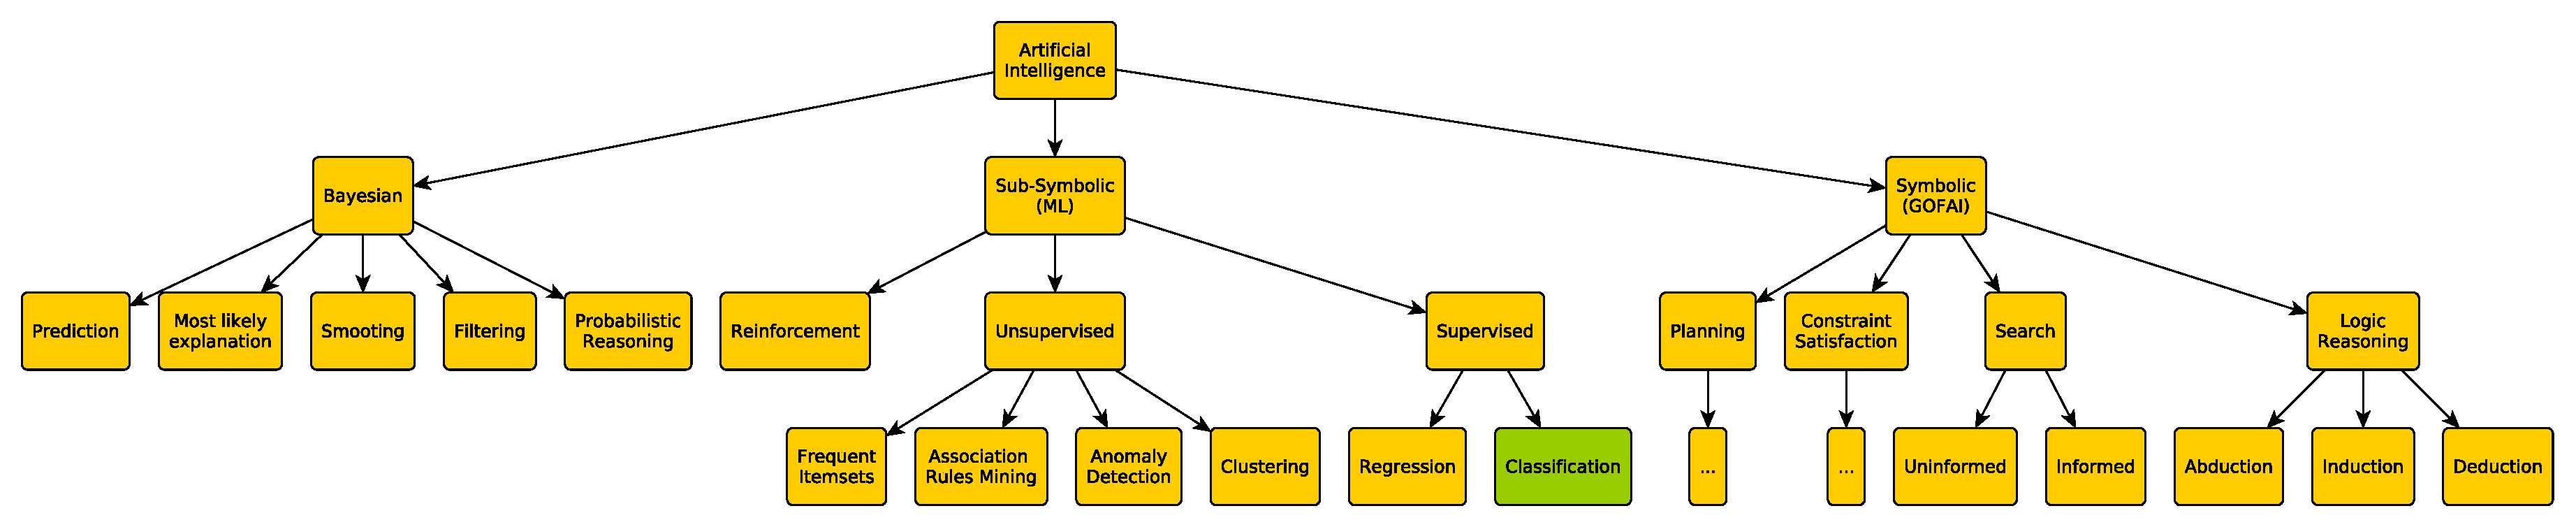
\includegraphics[width=.8\linewidth]{figures/random-image.pdf}
    \caption{Some random image}
    \label{fig:random-image}
\end{figure}

\section{Some cool topic}

%----------------------------------------------------------------------------------------
\chapter{Contribution}
\label{chap:contribution}
%----------------------------------------------------------------------------------------

You may also put some code snippet (which is NOT float by default), eg: \cref{lst:random-code}.

\lstinputlisting[float,language=Java,label={lst:random-code}]{listings/HelloWorld.java}

\section{Fancy formulas here}

%----------------------------------------------------------------------------------------
\chapter{Evaluation and Testing}
\label{chap:evaluation}
%----------------------------------------------------------------------------------------

%----------------------------------------------------------------------------------------
\chapter{Conclusion and Future works}
\label{chap:conclusion}
%----------------------------------------------------------------------------------------

%----------------------------------------------------------------------------------------
% BIBLIOGRAPHY
%----------------------------------------------------------------------------------------

\backmatter

\nocite{*} % Remove this as soon as you have the first citation

\bibliographystyle{alpha}
\bibliography{bibliography}

\begin{acknowledgements} % this is optional
Optional. Max 1 page.
\end{acknowledgements}

\end{document}
